\chapter{Exercises}

\section{Exercise 1: Wheatstone Bridge}

\subsection{Objective}
The objective of this exercise is to build and analyze the Wheatstone Bridge circuit and measure the resistance values using a multimeter.

\subsection{Equipment}

\begin{itemize}
    \item Digital multimeter
    \item Breadboard
    \item Resistors (2$\times$1k$\Omega$, 2$\times$2.2k$\Omega$, 1$\times$10k$\Omega$)
    \item Potentiometer (5k$\Omega$)
    \item Pover supply (5V)
    \item Wires and connectors
\end{itemize}

\newpage
\thispagestyle{plain}

\subsection{Procedure}

\begin{enumerate}
    \item We analysed the Wheatstone Bridge circuit theoretically and calculated the expected values based on the provided circuit configurations and component values.
    \begin{figure}[h]
        \centering
        \begin{circuitikz} \draw
            (0,4) to [battery, l=$V_{in}$] (0,0)
            (0,4) -- (4,4)
            node[label={[font=\footnotesize]right:A}] {}
            (4,4) to [R, l=$R_1$] (2,2)
            node[label={[font=\footnotesize]left:C}] {}
            (2,2) to [R, l=$R_2$] (4,0)
            node[label={[font=\footnotesize]right:B}] {}
            (4,0) to [R, l=$R_x$] (6,2)
            node[label={[font=\footnotesize]right:D}] {}
            (6,2) to [vR, l=$R_3$] (4,4)
            (4,0) -- (0,0)
            ;
        \end{circuitikz}
        \caption{Wheatstone Bridge circuit}
        \label{fig:wheatstone-bridge}
    \end{figure}
    
    Let's try to derive Wheatstone balance equation to find $R_x$:
    
    \begin{align*}
        V_{out} = V_C - V_D &= V_{R_2} - V_{R_x} = 0 \\
        R_C = \frac{R_2}{R_1+R_2} \quad &\text{and} \quad R_D = \frac{R_x}{R_3+R_x} \\
        \text{At balance,} \quad R_C &= R_D \\
        \frac{R_2}{R_1+R_2} &= \frac{R_x}{R_3+R_x} \\
        R_2(R_3+R_x) &= R_x(R_1+R_2) \\
        R_2R_3 + R_2R_x &= R_x R_1 + R_x R_2 \\
        R_2R_3 &= R_xR_1 \\
        R_x &= \boxed{\frac{R_2R_3}{R_1}}
    \end{align*}

    \newpage
    \thispagestyle{plain}

    \item Then, we have simulated the Wheatstone Bridge circuit in LTspice. The circuit is shown in Figure \ref{fig:ltspice}. The simulation results are shown in Table \ref{table:ltspice-results}. The simulation results show that the output voltage is zero when the bridge is balanced. The output voltage increases as the bridge becomes unbalanced.

    \begin{figure}[h]
        \centering
        \includegraphics[width=0.7\textwidth]{assets/ltspice.png}
        \caption{LTspice simulation of the Wheatstone Bridge}
        \label{fig:ltspice}
    \end{figure}
    
    \begin{table}[h]
        \centering
        \begin{tabular}{|
            >{\columncolor[HTML]{FFCCC9}}l 
            >{\columncolor[HTML]{FFCCC9}}l |
            >{\columncolor[HTML]{FFFC9E}}l 
            >{\columncolor[HTML]{FFFC9E}}l |}
            \hline
            \multicolumn{2}{|l|}{\cellcolor[HTML]{FD6864}For $R_x$ = 2.2k}                      & \multicolumn{2}{l|}{\cellcolor[HTML]{FFCC67}For $R_x$ = 1k}                        \\ \hline
            \multicolumn{1}{|l|}{\cellcolor[HTML]{FD6864}$R_b$} & \cellcolor[HTML]{FD6864}$V_{12}$ & \multicolumn{1}{l|}{\cellcolor[HTML]{FFCC67}$R_b$} & \cellcolor[HTML]{FFCC67}$V_{12}$ \\ \hline
            \multicolumn{1}{|l|}{\cellcolor[HTML]{FFCCC9}1k}   & 0                             & \multicolumn{1}{l|}{\cellcolor[HTML]{FFFC9E}1k}   & 0.10274                       \\ \hline
            \multicolumn{1}{|l|}{\cellcolor[HTML]{FFCCC9}2.2k} & 0.146536                      & \multicolumn{1}{l|}{\cellcolor[HTML]{FFFC9E}2.2k} & 0.258621                      \\ \hline
            \multicolumn{1}{|l|}{\cellcolor[HTML]{FFCCC9}3k}   & 0.216535                      & \multicolumn{1}{l|}{\cellcolor[HTML]{FFFC9E}3k}   & 0.330189                      \\ \hline
            \multicolumn{1}{|l|}{\cellcolor[HTML]{FFCCC9}4k}   & 0.284483                      & \multicolumn{1}{l|}{\cellcolor[HTML]{FFFC9E}4k}   & 0.397959                      \\ \hline
            \multicolumn{1}{|l|}{\cellcolor[HTML]{FFCCC9}5k}   & 0.337423                      & \multicolumn{1}{l|}{\cellcolor[HTML]{FFFC9E}5k}   & 0.44964                       \\ \hline
            \end{tabular}
        \caption{LTspice simulation results of the Wheatstone Bridge circuit}
        \label{table:ltspice-results}
    \end{table}

    \item We have theoretically calculated the expected resistance values for the Wheatstone Bridge circuit and check if the values verify the theoretical analysis.
    \begin{figure}[h]
        \centering
        \begin{circuitikz} \draw
            (0,4) to [battery, l=$V_{in}$] (0,0)
            (0,4) -- (4,4)
            node[label={[font=\footnotesize]right:A}] {}
            (4,4) to [R, l=1k] (2,2)
            node[label={[font=\footnotesize]left:C}] {}
            (2,2) to [R, l=1k] (4,0)
            node[label={[font=\footnotesize]right:B}] {}
            (4,0) to [R, l=$R_x$] (6,2)
            node[label={[font=\footnotesize]right:D}] {}
            (6,2) to [vR, l=2.2k] (4,4)
            (4,0) -- (0,0)
            ;
        \end{circuitikz}
        \caption{Wheatstone Bridge circuit}
        \label{fig:wheatstone-bridge}
    \end{figure}
    
    \newpage
    \thispagestyle{plain}

    If we apply the balance equation (Where $V_{CD} = 0$) we can find the value of $R_x$ which should be $2.2k$ according to LTspice result:
    
    \begin{align*}
        R_x &= \frac{R_2R_3}{R_1} \\
        R_x &= \frac{1k \times 2.2k}{1k} \\
        R_x &= 2.2k
    \end{align*}
    
    The LTspice results are consistent with the theoretical results.
    
    \item We have built the Wheatstone Bridge circuit on the breadboard according to the Figure \ref{fig:wheatstone-bridge-design} where $R_x = 2.2k\Omega$. We have connected the power supply to the circuit and measured the potential difference between C and D ($V_{CD}$) using a multimeter. We have adjusted the potentiometer to balance the bridge and measured the resistance value using a multimeter.

    \begin{figure}[h]
        \centering
        \begin{circuitikz} \draw
            (0,4) to [battery, l=$V_{in}$] (0,0)
            (0, 4) to [R, l=10k] (4, 4)
            node[label={[font=\footnotesize]right:A}] {}
            (4,4) to [R, l=1k] (2,2)
            node[label={[font=\footnotesize]left:C}] {}
            (2,2) to [vR, l=5k] (4,0)
            node[label={[font=\footnotesize]right:B}] {}
            (4,0) to [R, l=$R_x$] (6,2)
            node[label={[font=\footnotesize]right:D}] {}
            (6,2) to [R, l=2.2k] (4,4)
            (4,0) -- (0,0)
            ;
        \end{circuitikz}
        \caption{Wheatstone Bridge circuit}
        \label{fig:wheatstone-bridge-design}
    \end{figure}

    \begin{figure}[h]
        \centering
        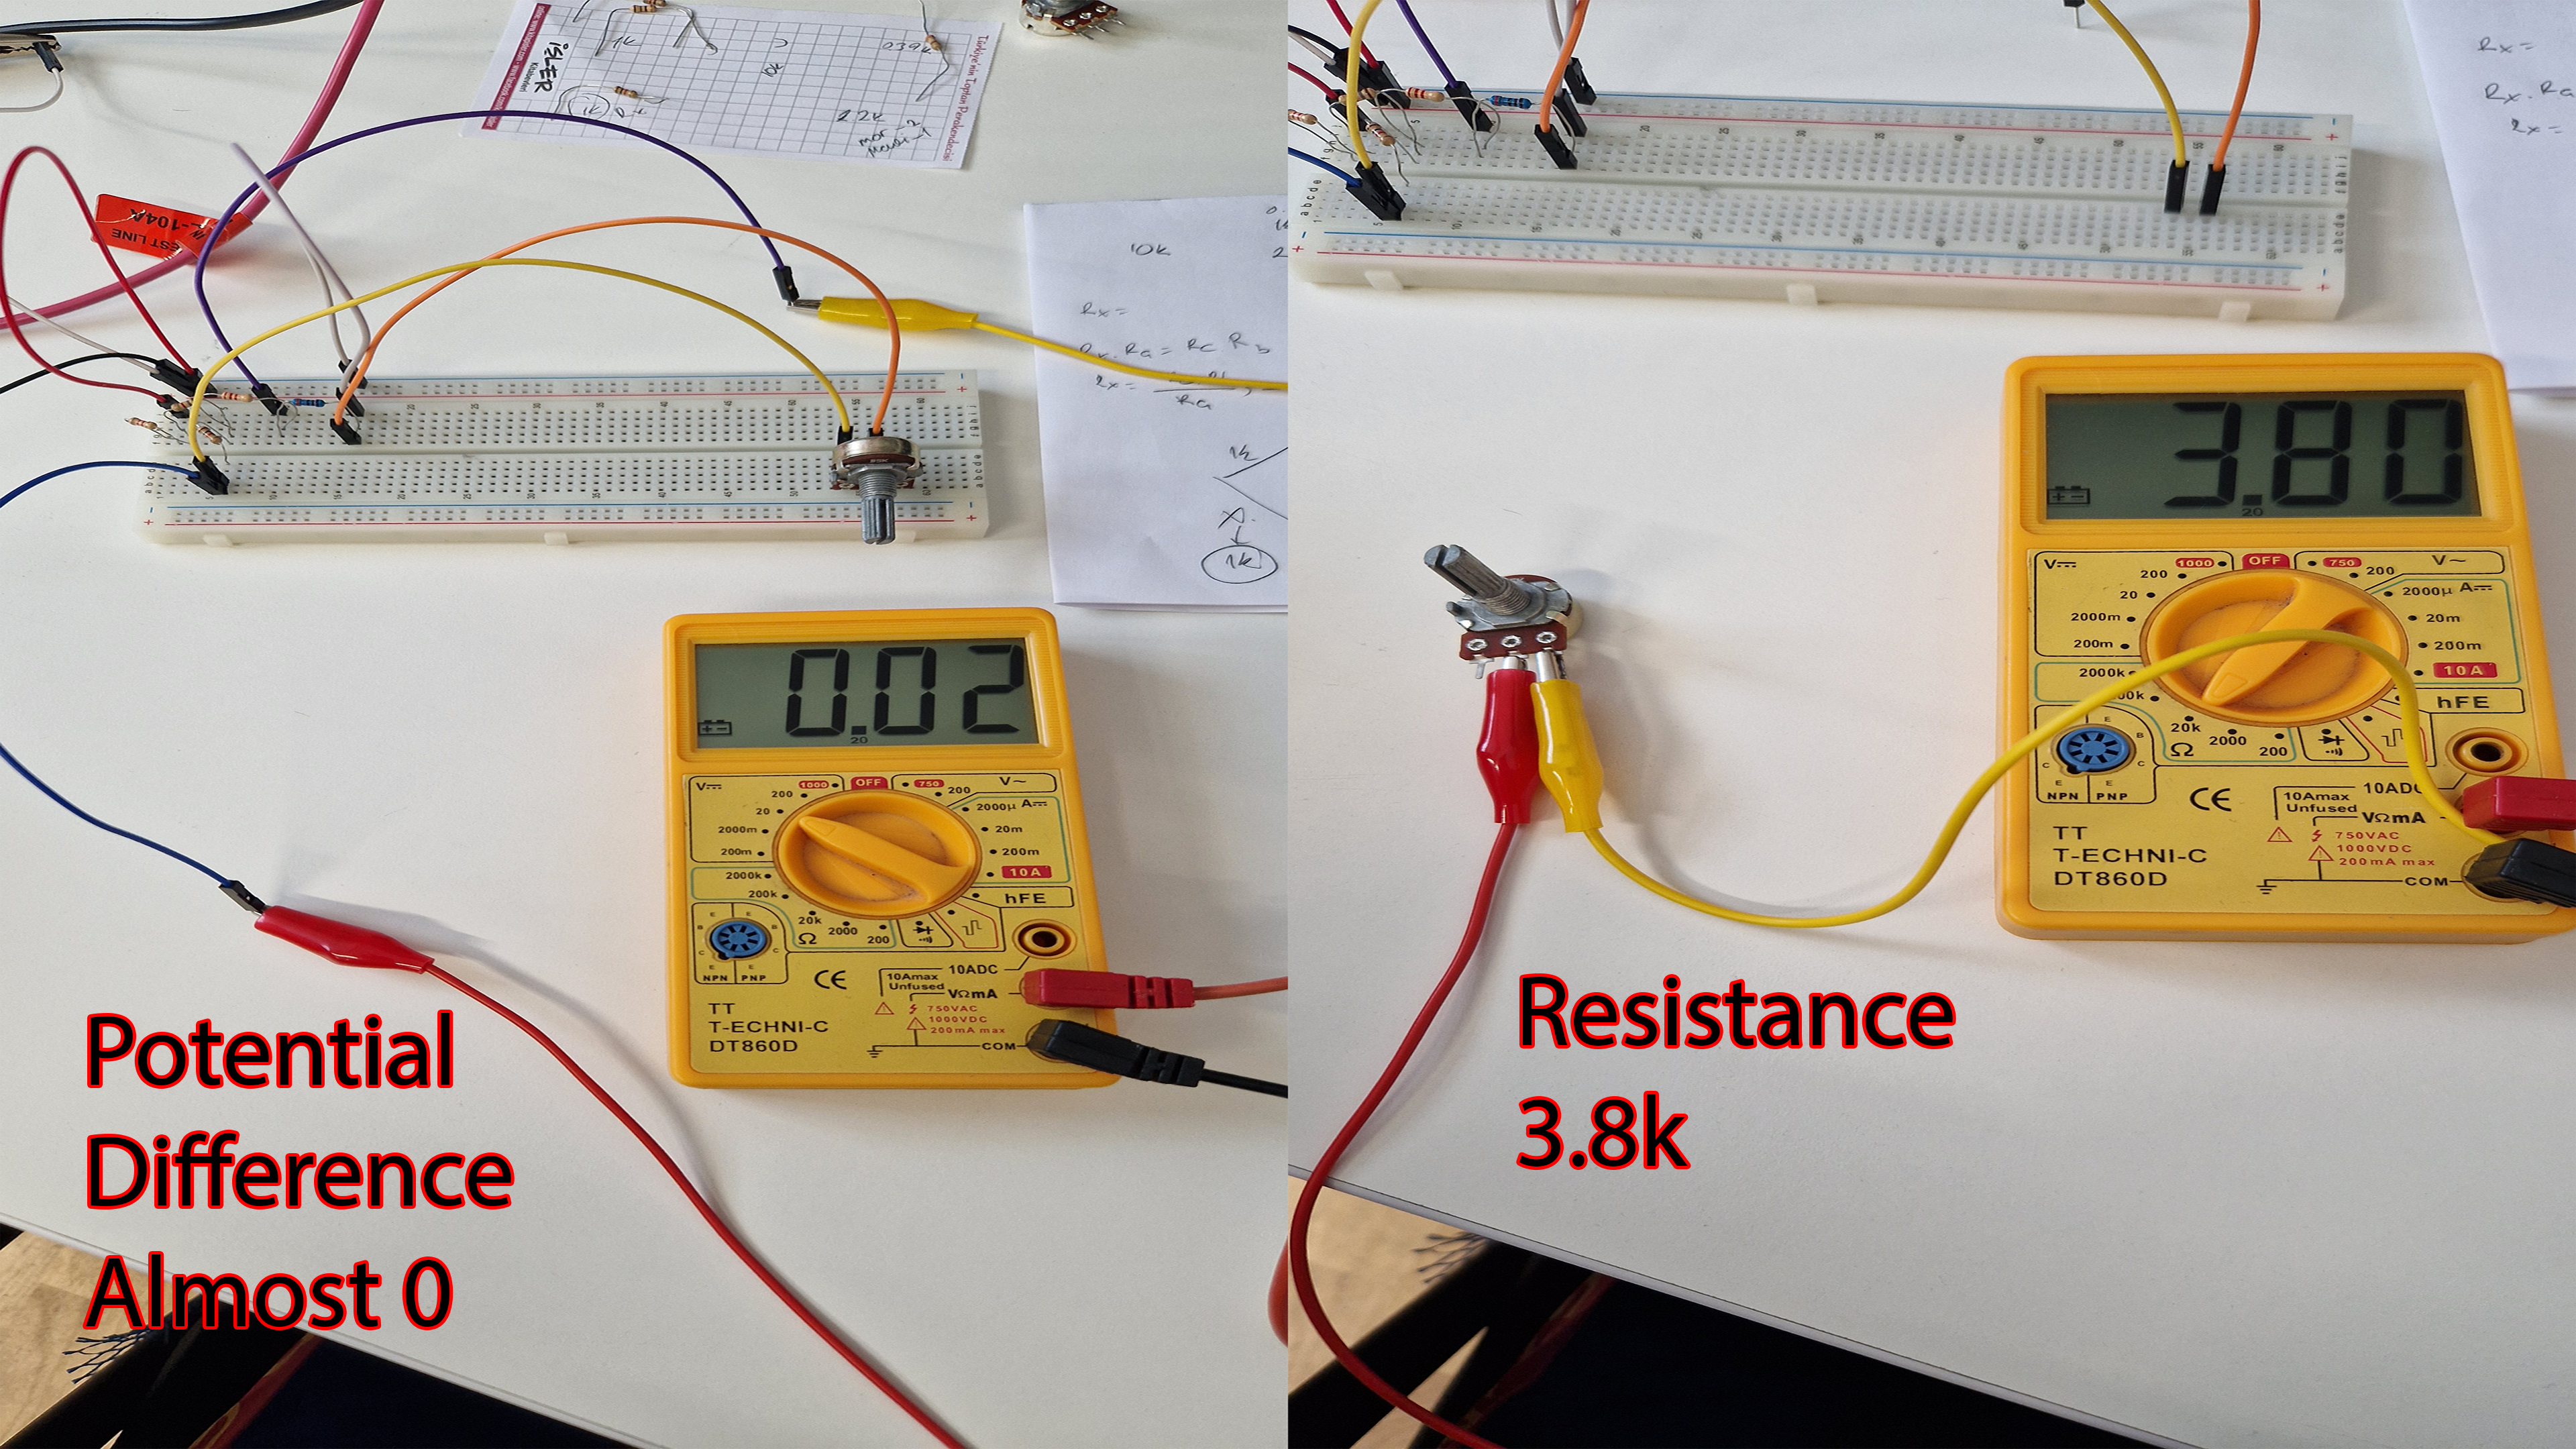
\includegraphics[width=0.7\textwidth]{assets/res-1.png}
        \caption{Balanced Wheatstone Bridge}
    \end{figure}

    We have measured the voltage and resistance values of the circuit and compared the results with the theoretical values. The results are close to the theoretical values. The differences between the theoretical and experimental values are due to the tolerance of the resistors, non-ideal cables and the measurement errors.

    \newpage
    \thispagestyle{plain}

    \item We have changed the value of $R_x$ to 1k$\Omega$ and repeated the measurements.
    
    \begin{figure}[h]
        \centering
        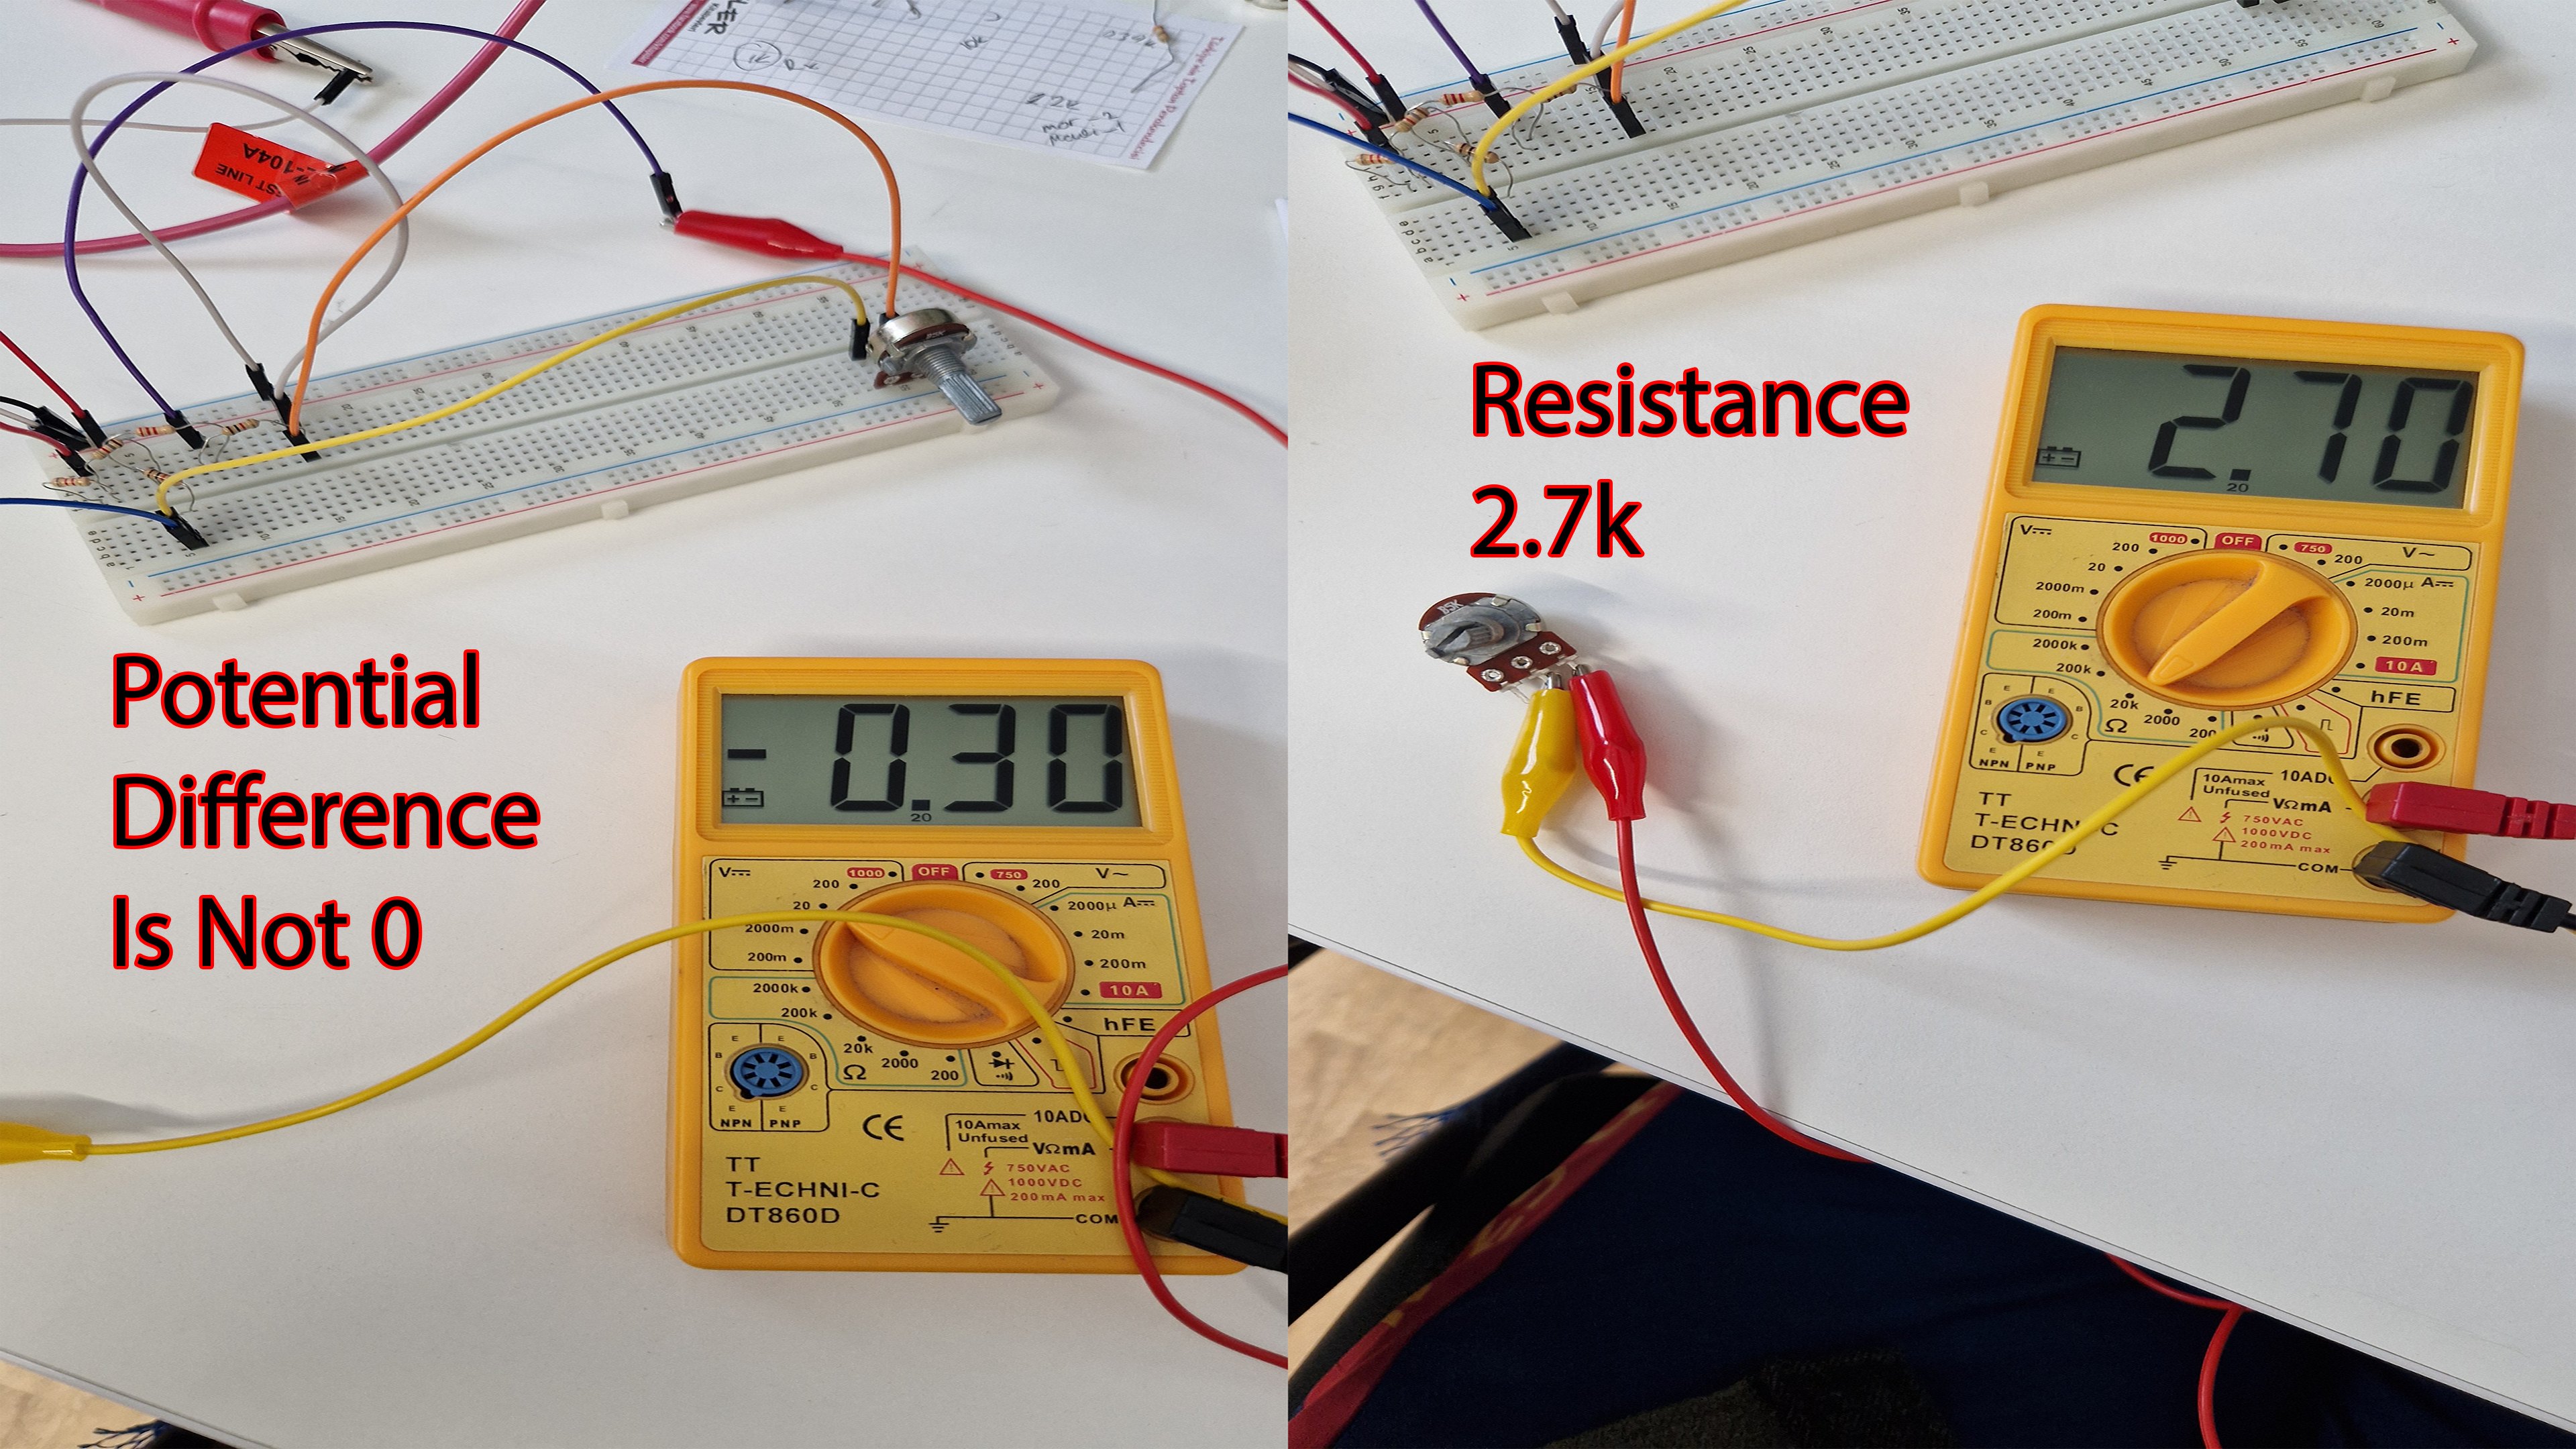
\includegraphics[width=0.7\textwidth]{assets/res-2.png}
        \caption{Unbalanced Wheatstone Bridge}
    \end{figure}

    When the circuit is not balanced, we can not apply the balance equation but if we apply the balance equation (Where $V_{CD} = 0$) we can find the theoretical value of $R_x$:
    
    \begin{align*}
        R_x &= \frac{R_2R_3}{R_1} \\
        R_x &= \frac{2.7k \times 2.2k}{1k} \\
        R_x &= 5.94k
    \end{align*}

    According to this setup and the theoretical calculations, the expected value of $R_x$ should be 5.94k$\Omega$ instead of 1k$\Omega$.
\end{enumerate}

\subsection{Results}

We have built the Wheatstone Bridge and measured the resistance values using a multimeter. Compared the results with the theoretical values and observed that the results are close to the theoretical values. The differences between the theoretical and experimental values are due to the tolerance of the resistors, non-ideal cables and the measurement errors.
